\section{Reuniones iniciales con los clientes y especificación inicial}

La reunión inicial fue con Juan Francisco Sanjuan Estrada quien explicó los distintos objetivos que se tenía pensado para la aplicación y los puntos de vista de los técnicos. Quienes utilizaban hojas de cálculo para gestionar el inventario y registrar los préstamos.
\\Dentro de las hojas de cálculo se detallaban exhaustivamente los objetos y también se indicaban sus ubicaciones actuales dentro del Edificio Científico Técnico III.
\\El problema es que esto no estaba tan organizado como parecía en un principio debido a que la gestión no la realizaba únicamente un técnico sino que eran tres. Es decir, había tres filosofías distintas a la hora de ir gestionando una parte del inventariado del Departamento de Informática.
\\Después de estas aclaraciones Juan comentó que no tenían un diseño en mente en el Departamento por lo que las propuestas iniciales de diseño iban a ser libres siempre y cuando se satisfacieran los requisitos principales de esta como la adición y eliminación del inventario y la concesión de préstamos.
\vspace{\baselineskip}
\\Luego de esta primera reunión se acordó en que podrían visualizarse los archivos Excel de los técnicos. Estos compartieron sus ficheros y desde ahí se pudo empezar a realizar la definición de los diferentes campos que irían ligados a cada tabla en la base de datos. Desde este punto se haría una propuesta inicial.
\\La propuesta inicial fue la de la figura \ref{diseno_principal_base_datos}.

\begin{figure}[ht]
    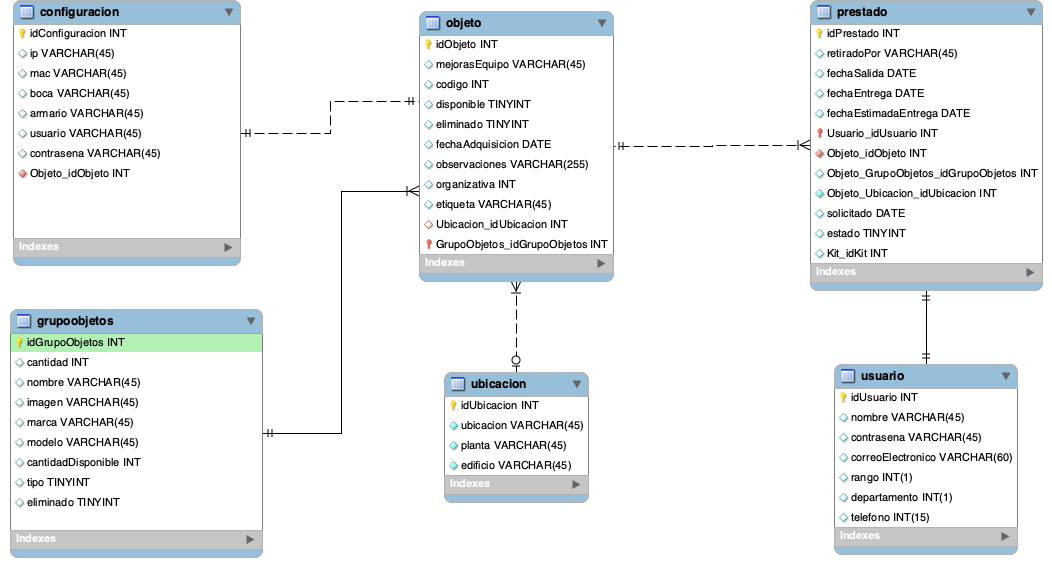
\includegraphics[width=\textwidth,height=\textheight,keepaspectratio]{db_old_design.png}
    \caption{Diseño principal de la base de datos}\label{diseno_principal_base_datos}
\end{figure}

La lógica de la aplicación consistiría en generar un grupo de objetos de un determinado tipo, inventario o fungible, 1 o 0. Dentro de este se contendrían objetos que irían vinculados a una ubicación. También los objetos podrían contener una posible configuración.
\\Esta configuración ¿para qué sirviría? Resulta que los técnicos aparte de manejar el inventariado disponible en la universidad también manejan las claves y accesos a esos determinados objetos, como puede ser el armario donde se ubiquen, sus direcciones mac o ip, las bocas de conexión con las regletas y más.
\\Este objeto tendría la posibilidad de tener varios préstamos, aunque es verdad que sería uno activo por persona, siempre dejando un registro de los anteriores usos que se hayan realizado del mismo. Este préstamo tendría que ir ligado obligatoriamente a un usuario. Contiene un campo de ``retiradoPor'' en el caso de que un docente o investigador quiera realizar un préstamo para su alumno.
\vspace{\baselineskip}
\\La propuesta inicial fue aceptada por el grupo de los técnicos y por el director del proyecto así que se pudo continuar a las siguientes etapas. Más adelante se realizaron unas modificaciones en los datos que manejarían los objetos por lo que las columnas de las tablas expuestas no serían las definitivas.
\\Se prepararon las propuestas iniciales de diseño mediante la utilización de la herramiento de Adobe XD. El aprendizaje de la herramienta es rápido y fácil de usar. Adobe XD le dió un toque de frescura y profesionalidad a las propuestas de diseño.
\\Las propuestas iniciales fueron ligadas a un diseño móvil ya que desde el primer momento se buscó que la aplicación fuera responsive, es decir, que desde un dispositivo móvil fuera fácil poder utilizarla. Esto influyó luego a la hora de realizar el diseño ya que se basó en un funcionamientos de ``cards'', es decir, componentes web con forma de carta y con fácil adaptabilidad a diseños móviles.
\\El esquema de navegación de la propuesta inicial quedaría tal como se puede observar en la Figura \ref{diseno_principal_sistema_navegacion}.
\\Donde se tienen dos roles de usuario, un personal docente o investigador y un técnico. Después del análisis hecho en la entrevista y correos mantenidos más tarde con el cliente se obtuvo el siguiente resultado de la Figura \ref{funcionamiento_principal_casos_de_uso}.

\begin{figure}[ht]
    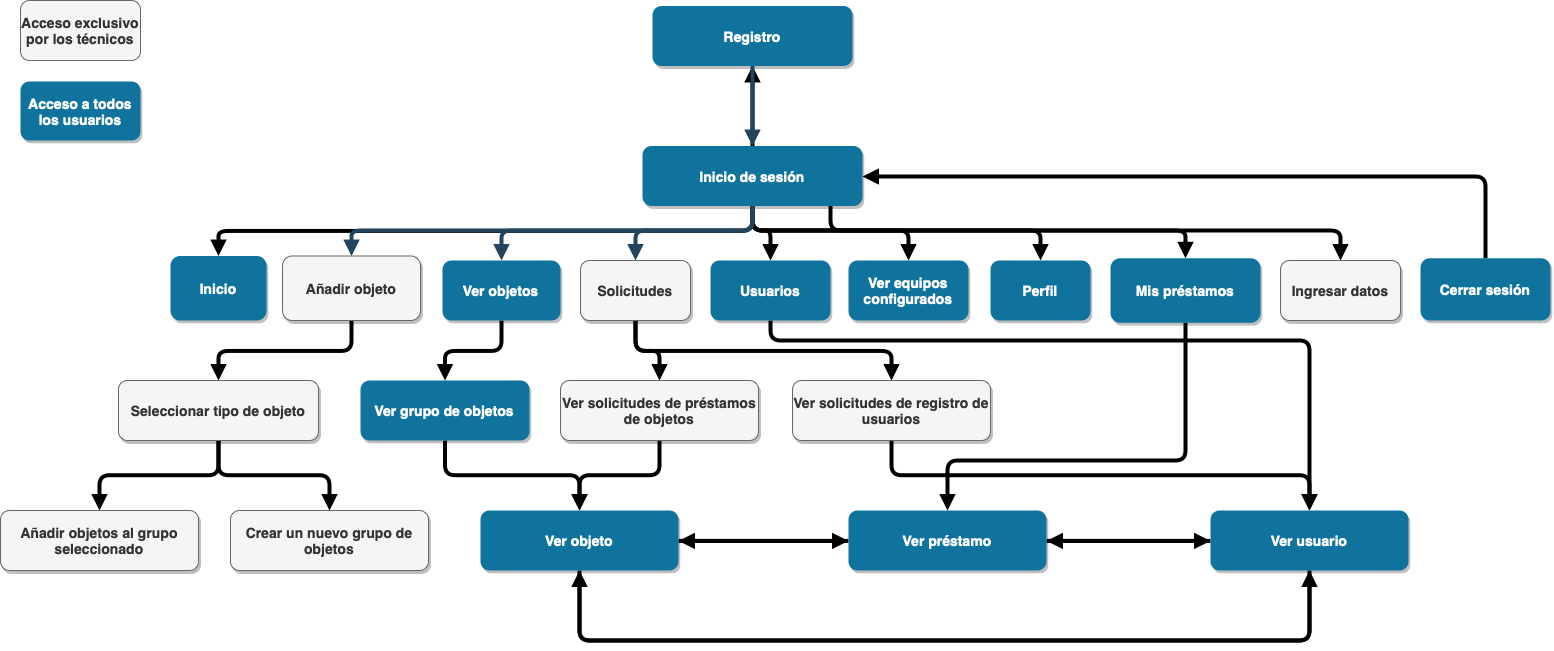
\includegraphics[width=\textwidth,height=\textheight,keepaspectratio]{flujo_de_navegacion.png}
    \caption{Diseño principal del sistema de navegación}\label{diseno_principal_sistema_navegacion}
\end{figure}

\begin{figure}[ht]
    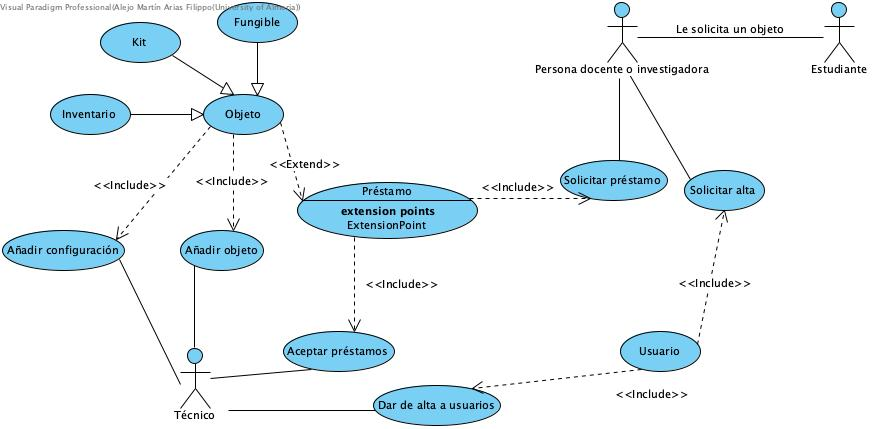
\includegraphics[width=\textwidth,height=\textheight,keepaspectratio]{../../diagramas/visual_paradigm/funcionamiento_principal.jpg}
    \caption{Diagrama de casos de uso del funcionamiento principal de la herramienta Inventarium}\label{funcionamiento_principal_casos_de_uso}
\end{figure}


\subsection{Inicio de sesión y registro}

El registro del usuario no conllevaba un registro instantáneo del mismo ya que este tiene que ser dado de alta por un técnico del sistema. Pueden observarse los diseños en la figura \ref{inicio_registro_design}.

\begin{figure}[ht]
    \begin{center}
        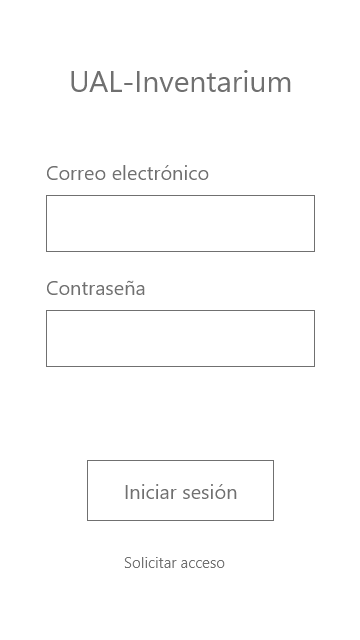
\includegraphics[scale=0.3]{web_design_adobe_xd/inicio_de_sesion.png}
        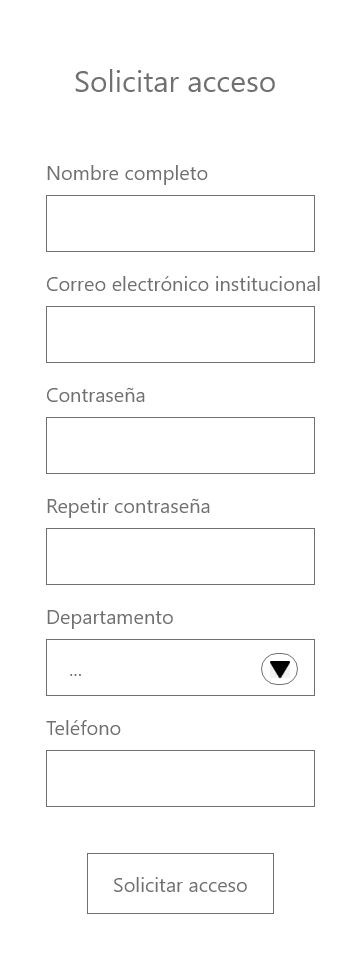
\includegraphics[scale=0.3]{web_design_adobe_xd/registro.png}
        \caption{Diseño del inicio de sesión y del registro}\label{inicio_registro_design}
    \end{center}
\end{figure}

Dentro del inicio de sesión se puede ver un campo interesante a considerar y es el de departamento. Una de las solicitudes que hizo el director del proyecto era poder agrupar a los usuarios dentro de departamentos. En este caso refiriéndose a dentro del personal docente e investigador que pertenecen al Departamento de Informática.
\\Los valores del departamento en la base de datos pueden ser los siguientes:

\begin{itemize}
    \item 0 = Departamento de informática (valor por defecto).
    \item 1 = Ingeniería de sistemas y automática.
    \item 2 = Lenguaje y sistemas informáticos.
    \item 3 = Ciencias de la computación e inteligencia artificial.
    \item 4 = Arquitectura y tecnología de computadores.
\end{itemize}

Otro campo para comprobar es el del correo electrónica institucional teniendo que ser este con la extensión \textbf{@inlumine.ual.es} o \textbf{@ual.es}.

\subsection{Barra de navegación}

La barra de navegación vertical tuvo una pequeña modificación que era incorporar una pequeña sección de inicio donde aparecieran información pertinente y relevante para el usuario. Esto será explicado más adelante en la parte de desarrollo. Puede observarse en la figura \ref{barra_de_navegacion}.

\begin{figure}[ht]
    \begin{center}
        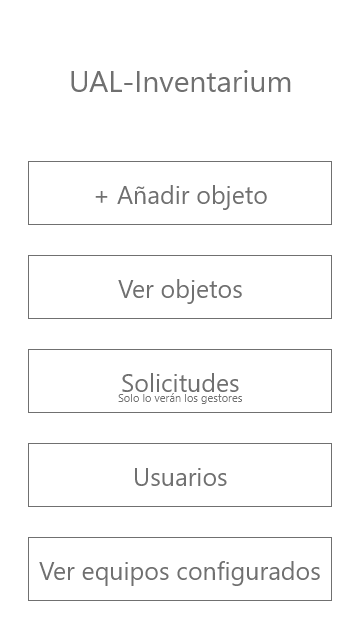
\includegraphics[scale=0.5]{web_design_adobe_xd/menu_principal.png}
        \caption{Diseño de la barra lateral de búsqueda}\label{barra_de_navegacion}
    \end{center}
\end{figure}

Dentro de ella se pueden ver cinco apartados que derivan en varios componentes visuales:

\begin{itemize}
    \item Añadir objeto: un acceso rápido donde poder añadir objetos dentro de grupos de objetos. Sección de menú solo visible para los técnicos.
    \item Ver objetos: apartado donde se visualizan los grupos de objetos, que contienen tanto el inventariado, fungibles y kits.
    \item Solicitudes: un menú donde se visualizan las solicitudes tanto de alta de usuarios como de objetos que le puedan llegar a los técnicos.
    \item Usuarios: componente visual donde cargan los usuarios registrados que hay dentro de la aplicación.
    \item Ver equipos configurados: aquí cargan únicamente objetos a los que se les haya aplicado una configuración. En caso de que no, no aparecerían.
\end{itemize}

\subsection{Añadir objeto}

\begin{figure}[ht]
    \begin{center}
        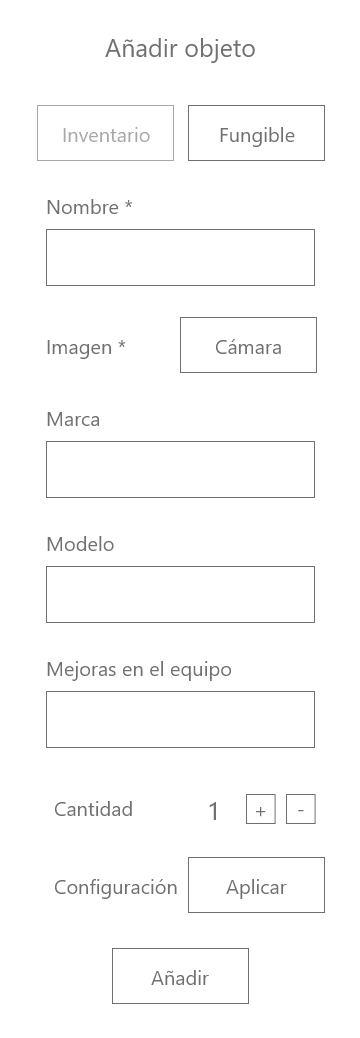
\includegraphics[scale=0.4]{web_design_adobe_xd/add_fungible.png}
        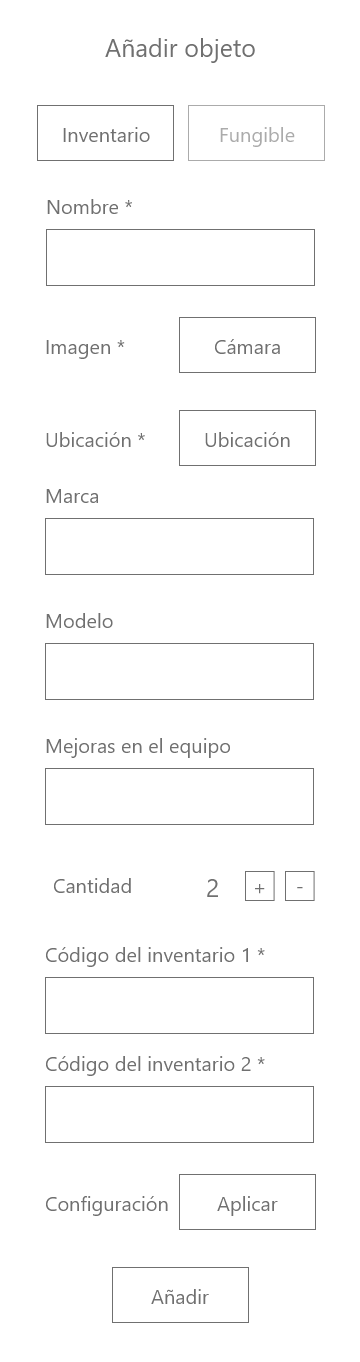
\includegraphics[scale=0.4]{web_design_adobe_xd/add_inventario.png}
        \caption{Diseño de la característica para poder añadir fungibles e inventarios}\label{adicion_inventario_fungible_design}
    \end{center}
\end{figure}

La única diferencia entre añadir un objeto de tipo inventario y otro fungible es que en el de inventario hay que registrar su código. Siempre que se vaya a añadir uno de estos elementos tiene que ser dentro de un \textbf{grupo de objetos} que debe haberse creado anteriormente. Por el resto, los dos son idénticos y se le puede añadir el mismo tipo de información. Estas diferencias se pueden observar en la figura \ref{adicion_inventario_fungible_design}.
\\No solo existen los fungibles e inventarios sino que también se solicitó más tarde poder crear kits.
\\Un \textbf{kit} puede considerarse como otro nivel de agrupación. Ya que un kit contiene más objetos dentro suyo que llamaremos ``objetos kit''. Para entender los niveles de agrupación puede observarse la figura \ref{jerarquia_grupo_objetos}.

\begin{figure}[ht]\resizebox{
        \linewidth}{!}{
        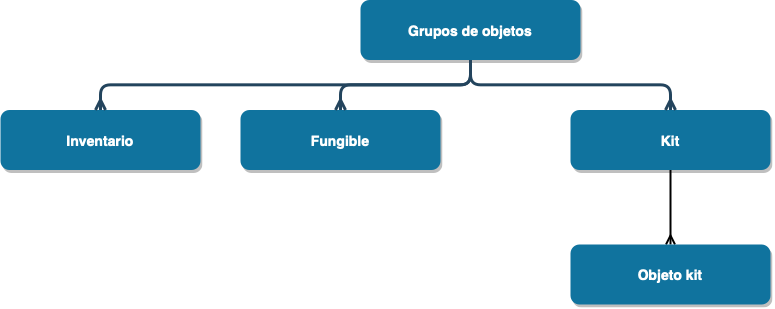
\includegraphics{jerarquia_grupo_objetos.png}
    }
    \caption{Jerarquía de elementos que derivan de grupo de objetos}\label{jerarquia_grupo_objetos}
\end{figure}

\subsection{Grupo de objetos y objetos}

Dentro de la sección de ``ver objetos'' de la barra de navegación se podrá observar la visualización de los grupos de objetos de la aplicación. En las cuales habrá también objetos. Estos dos conjuntos se pueden modificar y además se pueden pedir solicitudes para el inventariado, fungibles y kits. Pueden observarse en la figura \ref{grupo_objetos_y_objetos_design}.

\begin{figure}[ht]
    \centering
    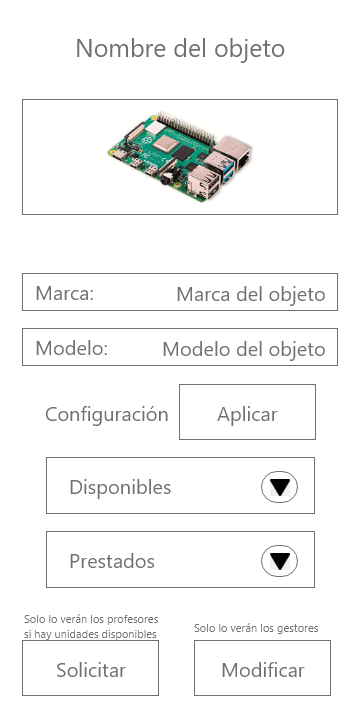
\includegraphics[scale=0.3]{web_design_adobe_xd/grupo_objetos.png}
    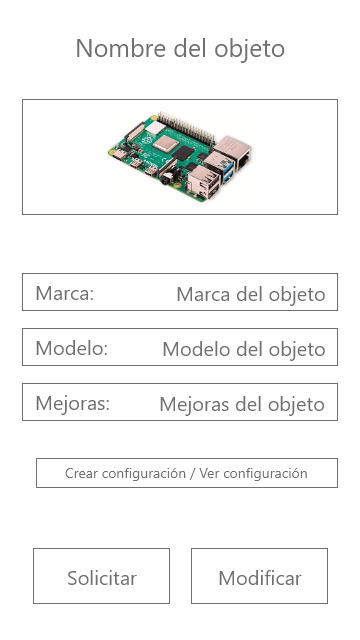
\includegraphics[scale=0.3]{web_design_adobe_xd/objeto_disponible.png}
    \caption{Grupo de objetos a la izquierda y objetos que contiene a la derecha}\label{grupo_objetos_y_objetos_design}
\end{figure}

\subsection{Usuarios}

En este apartado se podrán visualizar los usuarios que están registrados en la aplicación. Permitiéndose poder acceder a cada uno de los perfiles para ver sus respectivos datos y sus solicitudes o historial de préstamos. Tal como se observa en la figura \ref{grupo_usuarios_design}.


\begin{figure}[ht]
    \begin{minipage}{0.55\textwidth}
        \begin{center}
            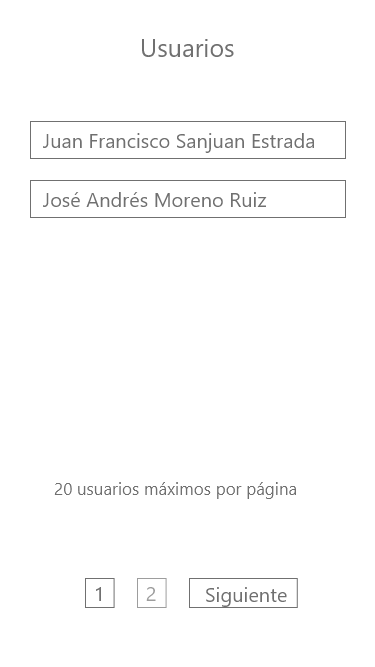
\includegraphics[scale=0.3]{web_design_adobe_xd/usuarios_buscados.png}
            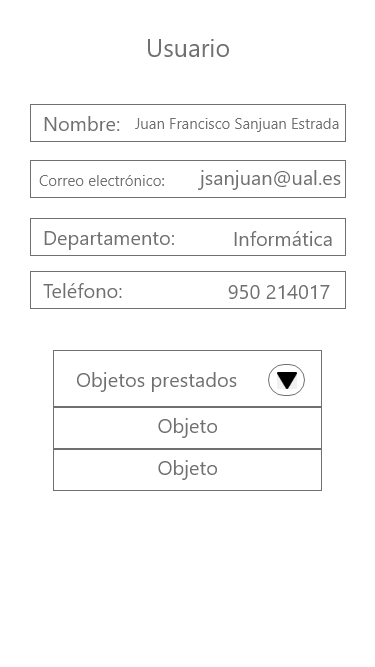
\includegraphics[scale=0.3]{web_design_adobe_xd/usuario.png}
            \caption{Grupo de usuarios a la izquierda y usuario único a la derecha}\label{grupo_usuarios_design}
        \end{center}
    \end{minipage}\hfill
    \begin{minipage}{0.35\textwidth}
        \centering
        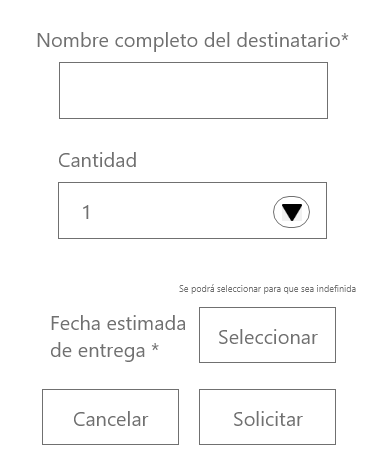
\includegraphics[scale=0.3]{web_design_adobe_xd/solicitar_prestamo.png}
        \caption{Solicitud del préstamo de un objeto}\label{solicitar_prestamos_design}
    \end{minipage}
\end{figure}
\subsection{Préstamos}

Los préstamos se pueden encontrar en tres diferentes estados:

\begin{itemize}
    \item Préstamo en curso: una solicitud de préstamo aprobada por un técnico y que está en vigencia.
    \item Préstamos solicitado: donde aparecerá una solicitud en espera a ser aprobada por un técnico, en el caso de que el objeto solicitado esté actualmente con un préstamo en curso no se permitirá conceder el préstamo solicitado hasta que finalice el actual.
    \item Préstamo finalizado: un préstamo en curso que ha sido devuelto, la aprobación de devolución la tiene que conceder un técnico.
    \item Préstamo vencido: un préstamo en curso que ha sobrepasado su fecha máxima que se había comprometido a devolver. En caso de que quiera solicitar una ampliación tiene que hacerlo nuevamente generando una nueva petición.
\end{itemize}

Cada solicitud irá con un color representativo dependiendo de cuál sea su estado, una utilidad tanto para el usuario como para el técnico que van a realizar las acciones de ir solicitando y concediendo préstamos. Tal como muestra la figura \ref{solicitar_prestamos_design}.


\subsection{Configuraciones}

Un objeto puede ir ligado a una información extra o no. Esta información no es algo que vuelva más descriptivo el objeto sino que es una utilidad que se solicitó en el momento del desarrollo de la aplicación. Su objetivo es poder acceder a información a la que suelen recurrir los técnicos de forma bastante frecuente. Como la IP o dirección MAC de un ordenador o las credenciales para poder acceder a él. Gracias a esta distinción se permite que la información de los equipos que disponen de una configuración en particular estén en una sección para ellos solos facilitándoles el acceso a ese recurso a los técnicos. Tal como se ve en la figura \ref{configuracion_design}.

\begin{figure}[ht]
    \centering
    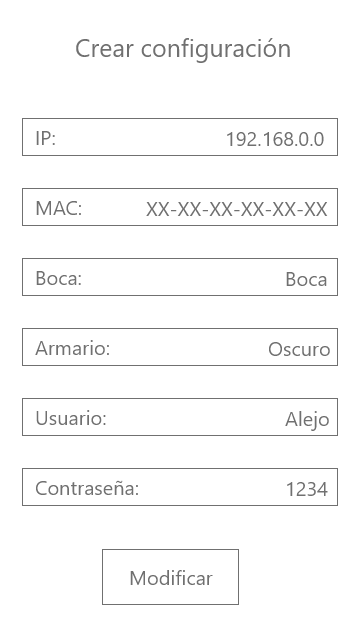
\includegraphics[scale=0.35]{web_design_adobe_xd/ver_configuracion.png}
    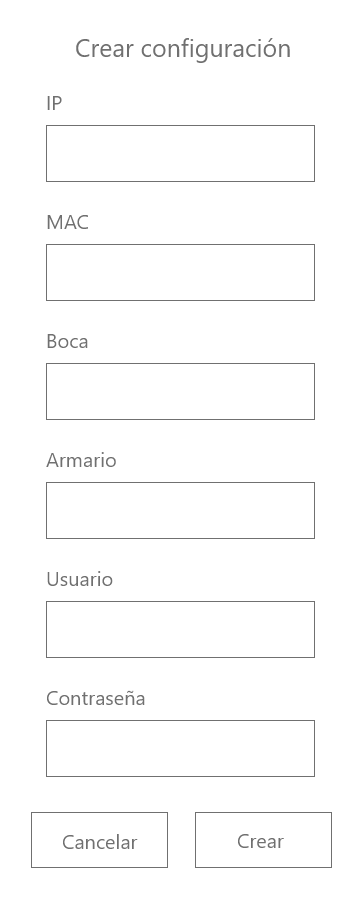
\includegraphics[scale=0.3]{web_design_adobe_xd/crear_configuracion.png}
    \caption{Visualización de los campos de configuración a la izquierda y creación de estos a la derecha}\label{configuracion_design}
\end{figure}